\chapter{Opciones y volatilidad}\label{cap:opciones}

\section{Black--Scholes y sus variantes}
Para una call europea con dividendo continuo $q$:
\begin{equation}
C = S e^{-qT}N(d_1) - K e^{-rT}N(d_2),\qquad d_{1,2}=\frac{\ln(S/K)+(r-q\pm\frac12\sigma^2)T}{\sigma\sqrt T},
\end{equation}
y la paridad put--call $C-P = Se^{-qT}-Ke^{-rT}$ (\py{options.bs\_price}). La misma fórmula cubre las tres clases de activo:
\begin{itemize}
\item \textbf{Acciones/índices}: $q$ = rentabilidad por dividendo.
\item \textbf{FX} (Garman--Kohlhagen): $q = r_{\text{extranjero}}$ (\py{garman\_kohlhagen}).
\item \textbf{Futuros de materias primas} (Black-76): $S=F$, $q=r$ (\py{black76}).
\end{itemize}

\section{Griegas}
\begin{table}[h]\centering\small
\begin{tabularx}{\textwidth}{llX}
\toprule
Griega & Fórmula (call) & Significado para el trader \\ \midrule
Delta & $e^{-qT}N(d_1)$ & Equivalente en subyacente; cobertura. \\
Gamma & $e^{-qT}\varphi(d_1)/(S\sigma\sqrt T)$ & Cuánto cambia la delta: el «convexo» que se compra. \\
Vega & $Se^{-qT}\varphi(d_1)\sqrt T$ & P\&L por punto de volatilidad implícita. \\
Theta & $\partial C/\partial t$ & Lo que se paga cada día por tener gamma. \\
Rho & $KTe^{-rT}N(d_2)$ & Sensibilidad a tipos. \\
\bottomrule
\end{tabularx}
\end{table}
La relación fundamental de una cartera cubierta en delta es
\begin{equation}
\text{P\&L diario} \approx \tfrac12\,\Gamma\,S^2\left(\hat\sigma^2_{\text{realizada}}-\sigma^2_{\text{implícita}}\right)\Delta t ,
\end{equation}
es decir, \textbf{comprar opciones es apostar a que la volatilidad realizada superará a la implícita}
y venderlas, lo contrario. Esto es el núcleo del trading de volatilidad.

\begin{figure}[h]\centering
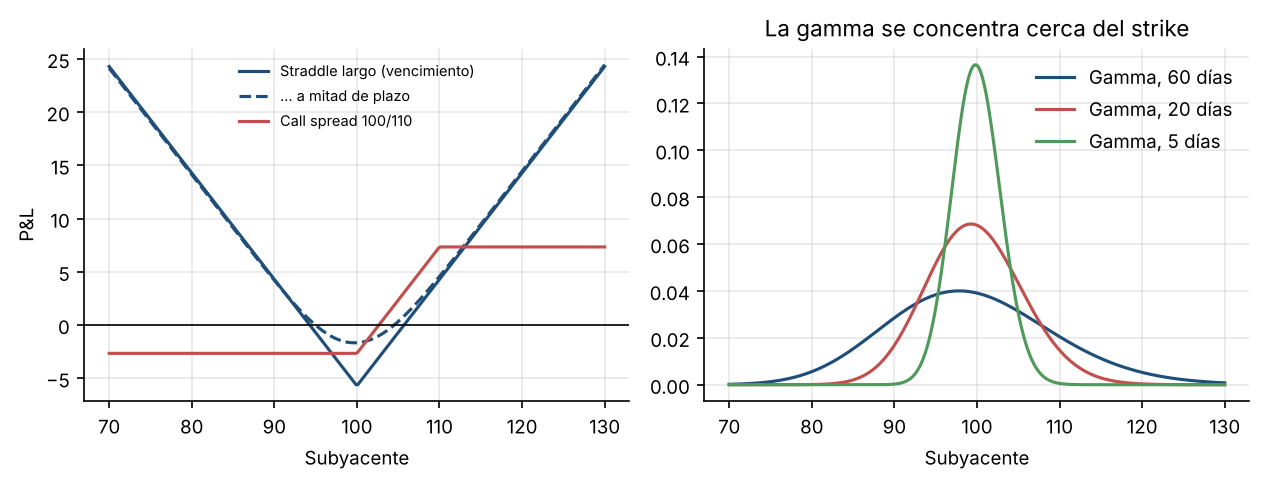
\includegraphics[width=\textwidth]{f11_opciones}
\caption{Izquierda: P\&L de un straddle largo y de un call spread. Derecha: la gamma se concentra
cerca del strike al acercarse el vencimiento.}
\end{figure}

\section{Volatilidad implícita y movimiento esperado}
La volatilidad implícita es la $\sigma$ que iguala el precio de mercado (\py{options.implied\_vol}).
El movimiento esperado a $1\sigma$ hasta una fecha es $S\,\sigma\sqrt{d/365}$
(\py{expected\_move}); el precio del straddle ATM dividido por $S$ ($\approx0{,}8\,\sigma\sqrt T$) es la
regla rápida para saber cuánto descuenta el mercado ante resultados o un dato macro.
\begin{lstlisting}
python scripts/calculadoras.py opcion --spot 100 --strike 105 --dias 30 --vol 25 --tipo-interes 4
python scripts/calculadoras.py movimiento --spot 5200 --vol 14 --dias 1
\end{lstlisting}

\paragraph{Sonrisa y estructura temporal.} En renta variable las puts bajistas tienen más volatilidad
implícita (\emph{skew}) por la demanda de protección; en FX la sonrisa es más simétrica y se cotiza en
\emph{risk reversals} y \emph{butterflies}; en materias primas a menudo el skew es alcista (miedo a
subidas de oferta escasa). La prima de varianza (implícita $>$ realizada en promedio) es la razón por la
que vender volatilidad es rentable\ldots{} con colas izquierdas muy gruesas (febrero de 2018).

\section{Estrategias básicas}
\begin{itemize}
\item \textbf{Call/put largas}: direccionales con pérdida acotada.
\item \textbf{Spreads verticales}: abaratan la prima a cambio de limitar la ganancia.
\item \textbf{Straddle/strangle}: largo volatilidad (comprado) o corto volatilidad (vendido).
\item \textbf{Covered call / cash-secured put}: venta de volatilidad sobre una posición o un objetivo de compra.
\item \textbf{Collar}: protección financiada vendiendo potencial alcista.
\item \textbf{Calendarios}: apuesta a la estructura temporal.
\end{itemize}

\begin{ejercicios}
\begin{enumerate}
\item Verifica la paridad put--call con \py{bs\_price} para varios strikes.
\item Una acción a 100 tiene el straddle ATM de 7 días a 5,60. ¿Qué movimiento descuenta el mercado? ¿Qué volatilidad implícita aproximada supone?
\end{enumerate}
\end{ejercicios}
